\chapter{recommendation for further work}
\section{Simlated environment}

	Furthemore, a framework to test and build an entire automated system is suggested. This framework includes a simulated 
	simulated envorinment, that realisicly makes it possible, to navigate a drone within an simulated environment. The environment 
	is based on the Roboter Operating System (ROS) and for the simulations the tum\_simulation ros package, developed by the Technische Universität 
	München, was resorted to. 
	
	
	ROS, as the name suggests, is a framework for a software infrastracture within a robot. With the right drivers installed, 
	it can access and use the robots hardware and serves as a messenger system between robot components. Ros packages make it easy to 
	reuse important functionalities. Gazebo on the other hand is a 3D dynamic simulator for robotics. It can accurately and efficiently simulate robots regarding
	their physics. 
	
	
	Thus, with the tum\_simulation package you can navigate an AR.drone 1.0 and 2.0 in different worlds created with a gazebo node. This drone is eqipped with a bottom camera 
	and a frot camera. The cameras each log their output to a ros topic. Additionally, message time stamps, the height sensor output, 
	battery percentage, position, rotation
	velocity and accelaration are also logged to rostopics. While the drone can also be navigated using a playstation 3 controller, as shown in figure 
	\ref{fig:tumsim}, showing a section of the tum\_simulation package content structure, 
	for an automated system, the drone should rather be addressed using the command line interface. For example 
	the command shown in sourcecode listing \ref{lst:drone_cmd} will make the drone fly foreward. 
	
	\begin{lstlisting}[language=bash, caption=drone navigation command, label=lst:drone_cmd]
    rostopic pub -r 10 /cmd_vel geometry_msgs/Twist  '{linear:  {x: 1.0, y: 0.0, z: 0.0}, angular: {x: 0.0,y: 0.0,z: 0.0}}'
	\end{lstlisting}
	
	\fig{img/tum_sim.png}{tum simulator setup. Source: $http://wiki.ros.org/tum_simulator$}{fig:tumsim}{0.8}
	
	By accessing the camera output of the drone via rostopics, SLAM algorithms can be applied on the generated images. Some SLAM-Algorithms, 
	such as an modified version of the ORB-SLAM-Algorithm (\href{https://github.com/rayvburn/ORB-SLAM2_ROS}{ORB\_SLAM2\_ROS}), publish the created pointcloud again in an own rostopic.
	The fight path planning algorithm on the other hand takes the publishes pointcloud as input and navigates the drone using the command line interface. 
	
	This circle of a fully automated SLAM system is shown in figure \ref{fig:autsys}. For the initialiazation of the process, the manual step of flying
	the drone may be required. This is because the ORB-SLAM system needs a translational movement to initialize the algorithm. Though, in most cases, 
	a normal take off will be sufficient. 
	
	\fig{img/aut_system.png}{Automated SLAM system}{fig:autsys}{0.8}
	
	In figure \cite{fig:simfigs} the simulated environment with gazebo can be found in figure a. Here, the drone (in black) is flying in front of the building. 
	The output of the front camera is shown in figure b. Therefore, the output calibration data of the front camera, such as the focal lengt, 
	can be found in an own rostopic. In figure c, the ORB-SLAM-Algorithm was applied to the output of the front camera. Green dots represent the 
	finding of an ORB-feature. 
	
	
	\begin{figure}%
    \centering
    \subfloat[\centering gazebo simulation]{{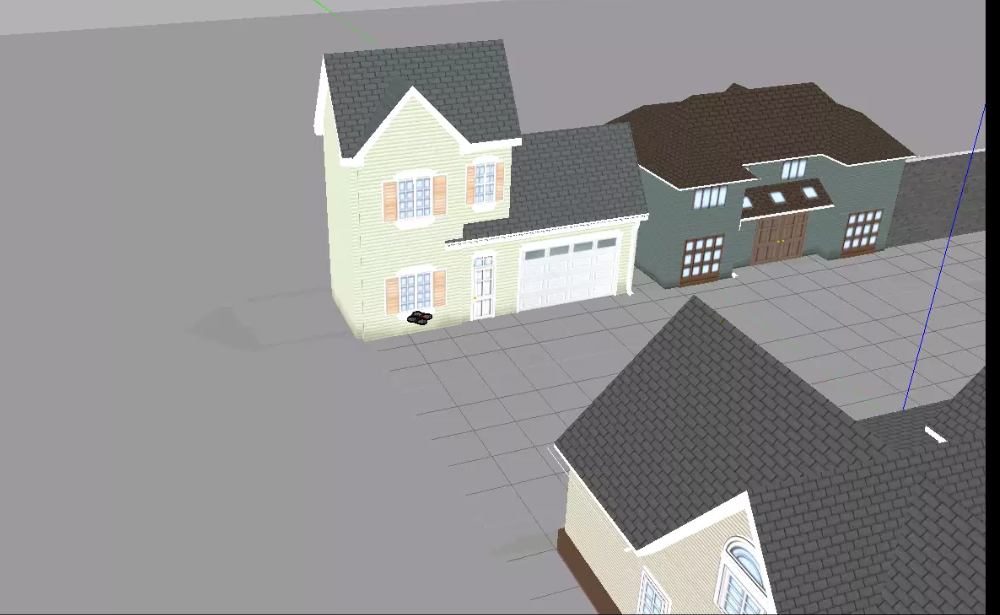
\includegraphics[width=5cm]{img/drohne_oben.png} }}%
    \qquad
    \subfloat[\centering front camera simulation]{{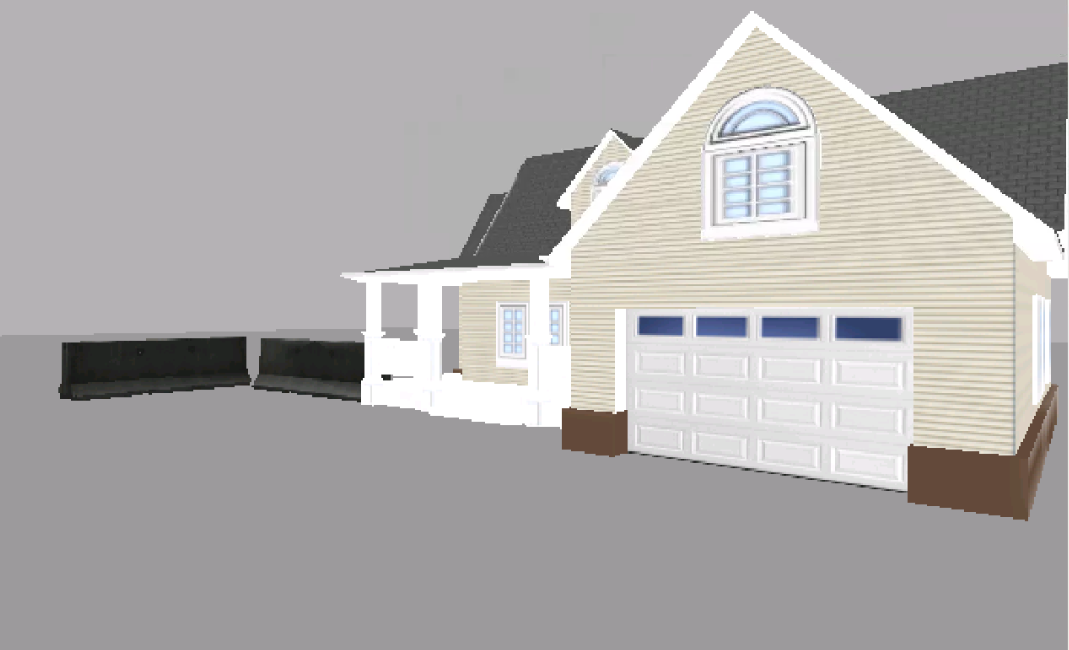
\includegraphics[width=5cm]{img/drohne_kamera.png} }}%
	\qquad
    \subfloat[\centering ORB applied on simulation]{{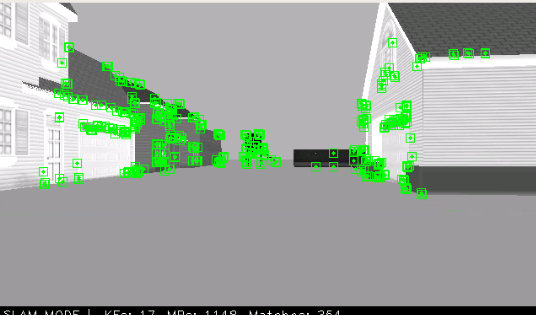
\includegraphics[width=5cm]{img/front_camera_orb.png} }}%
    \caption{
	The drone in a gazebo simulation in a), the output of the front camera of the drone in b) and
	the ORB-SLAM algorithm applied on the front camera output in with the detected ORB features marked green c).
	}%
    \label{fig:simfigs}%
	\end{figure}
	
	\subsection{Current setup}
	
	Currently the framework is set up in an environment provided by theconstructsim.com. This platform is enabling ROS-developers to program in preconfigured
	ROS-environments. The environment comes with the possibility to open terminal consols, a file management system, a simulator, that automatically 
	detects, when a gazebo simulation is running. Also, you have a graphical interface for other graphical applications, such as the viewer of ORB-SLAM.
	The current environments is set up with ROS kinetic and Ubuntu 16.04.6 LTS (Xenial). The tum\_simulator, ORB-SLAM and all of their dependencies are already installed. 
	
	\begin{lstlisting}[language=bash, caption=Launching the simulated environment, label=lst:sim_cmd]
# launch the gazebo simulation
roslaunch cvg_sim_gazebo ardrone_testworld.launch
	
# launch ORB-SLAM
rosrun ORB_SLAM2 Mono ${PATH_TO_VOCABULARY} ${PATH_TO_SETTINGS_FILE}
	
# takeoff with drone 
rostopic pub -1 /ardrone/takeoff std_msgs/Empty
	\end{lstlisting}
	
	In listing \ref{lst:sim_cmd} the commands for launching the gazebo simulation, ORB-SLAM and the drone are displayed. After launching thouse 
	applications, only the path planning algorithm based on the resulting point cloud is missing. However, multiple solutions for such algorithms 
	exist \cite{path}, appying it on the system is not part of this paper and will be done in further research. 
	
\section{Flight Path Planning algorithm}